\documentclass{article}
%%%%%%%%%%%%%%%%%%%%%%%%%%%%%%%%%%%%%%%%%%%%%%%%%%%%%%%%%%%%%%%%%%%%%%%%%%%%%%%%%%%%%%%%%%%%%%%%%%%%%%%%%
\usepackage{csquotes,xpatch}% recommended
\usepackage[backend=bibtex,
style=authoryear-comp,
sortcites=false,
maxbibnames=5,maxcitenames=2,
firstinits=true,
natbib=true,
]{biblatex}

\addbibresource{refs.bib}

% natbib = true: add comma between author and year
% firstinits: for first name initials in bibliography
\renewcommand{\postnotedelim}{ } % remove comma in post citation in autocite
%\addbibresource{refs.bib}
%%%%%%%%%%%%%%%%%%%%%%%%%%%%%%%%%%%%%%%%%%%%%%%%%%%%%%%%%%%%%%%%%%%%%%%%%%%%%%%%%%%%%%%%%%%%%%%%%%%%%%%%%

% Combine label and labelyear links
\xpatchbibmacro{cite}
{\usebibmacro{cite:label}%
	\setunit{\addspace}%
	\usebibmacro{cite:labelyear+extrayear}}
{\printtext[bibhyperref]{%
		\DeclareFieldAlias{bibhyperref}{default}%
		\usebibmacro{cite:label}%
		\setunit{\addspace}%
		\usebibmacro{cite:labelyear+extrayear}}}{}{}

% Include labelname in labelyear link
\xpatchbibmacro{cite}
{\printnames{labelname}%
	\setunit{\nameyeardelim}%
	\usebibmacro{cite:labelyear+extrayear}}
{\printtext[bibhyperref]{%
		\DeclareFieldAlias{bibhyperref}{default}%
		\printnames{labelname}%
		\setunit{\nameyeardelim}%
		\usebibmacro{cite:labelyear+extrayear}}}{}{}

% Access hyperref's citation link start/end commands
\makeatletter
\protected\def\blx@imc@biblinkstart{%
	\@ifnextchar[%]
	{\blx@biblinkstart}
	{\blx@biblinkstart[\abx@field@entrykey]}}
\def\blx@biblinkstart[#1]{%
	\blx@sfsave\hyper@natlinkstart{\the\c@refsection @#1}\blx@sfrest}
\protected\def\blx@imc@biblinkend{%
	\blx@sfsave\hyper@natlinkend\blx@sfrest}
\blx@regimcs{\biblinkstart \biblinkend}
\makeatother

\newbool{cbx:link}

% Include parentheses around labelyear in \textcite only in
% single citations without pre- and postnotes
\def\iflinkparens{%
	\ifboolexpr{ test {\ifnumequal{\value{multicitetotal}}{0}} and
		test {\ifnumequal{\value{citetotal}}{1}} and
		test {\iffieldundef{prenote}} and
		test {\iffieldundef{postnote}} }}

\xpatchbibmacro{textcite}
{\printnames{labelname}}
{\iflinkparens
	{\DeclareFieldAlias{bibhyperref}{default}%
		\global\booltrue{cbx:link}\biblinkstart%
		\printnames{labelname}}
	{\printtext[bibhyperref]{\printnames{labelname}}}}{}{}

\xpatchbibmacro{textcite}
{\usebibmacro{cite:label}}
{\iflinkparens
	{\DeclareFieldAlias{bibhyperref}{default}%
		\global\booltrue{cbx:link}\biblinkstart%
		\usebibmacro{cite:label}}
	{\usebibmacro{cite:label}}}{}{}

\xpretobibmacro{textcite:postnote}
{\ifbool{cbx:link}% patch 2.7+
	{\ifbool{cbx:parens}
		{\bibcloseparen\global\boolfalse{cbx:parens}}
		{}%
		\biblinkend\global\boolfalse{cbx:link}}
	{}}
{}
{\xpatchbibmacro{textcite}% patch earlier releases
	{\setunit{%
			\ifbool{cbx:parens}
			{\bibcloseparen\global\boolfalse{cbx:parens}}
			{}%
			\multicitedelim}}
	{\ifbool{cbx:link}
		{\ifbool{cbx:parens}
			{\bibcloseparen\global\boolfalse{cbx:parens}}
			{}%
			\biblinkend\global\boolfalse{cbx:link}}
		{}%
		\setunit{%
			\ifbool{cbx:parens}
			{\bibcloseparen\global\boolfalse{cbx:parens}}
			{}%
			\multicitedelim}}
	{}{}}
%%%%%%%%%%%%%%%%%%%%%%%%%%%%%%%%%%%%%%%%%%%%%%%%%%%%%%%%%%%%%%%%%%%%%%%%%%%%%%%%%%%%%%%%%%%%%%%%%%%%%%%%%
\DeclareNameAlias{sortname}{last-first} % last name first
\renewbibmacro{in:}{} % remove in: before journal

%%%%%%%%%%%%%%%%%%%%%%%%%%%%%%%%%%%%%%%%%%%%%%%%%%%%%%%%%%%%%%%%%%%%%%%%%%%%%%%%%%%%%%%%%%%%%%%%%%%%%%%%%
\usepackage{graphicx}
\usepackage{epstopdf} 
%%%%%%%%%%%%%%%%%%%%%%%%%%%%%%%%%%%%%%%%%%%%%%%%%%%%%%%%%%%%%%%%%%%%%%%%%%%%%%%%%%%%%%%%%%%%%%%%%%%%%%%%%
\usepackage{calrsfs}
\usepackage{physics}
\usepackage{mathtools}  
\usepackage{amsmath}
\usepackage{amssymb}
\usepackage{tabulary}
\usepackage{booktabs}
\usepackage{hyperref}
%%%%%%%%%%%%%%%%%%%%%%%%%%%%%%%%%%%%%%%%%%%%%%%%%%%%%%%%%%%%%%%%%%%%%%%%%%%%%%%%%%%%%%%%%%%%%%%%%%%%%%%%%
%\usepackage{chngcntr}
%\numberwithin{equation}{chapter}
%\counterwithin{figure}{chapter}
%%%%%%%%%%%%%%%%%%%%%%%%%%%%%%%%%%%%%%%%%%%%%%%%%%%%%%%%%%%%%%%%%%%%%%%%%%%%%%%%%%%%%%%%%%%%%%%%%%%%%%%%%
\setlength{\parindent}{2em}
\setlength{\parskip}{1em}

\linespread{1.6}
\usepackage{geometry}
\geometry{
	a4paper,
	total={134mm,225mm},
	left=38mm,
	top=35mm,
	headsep=.5in
}
\raggedbottom
%%%%%%%%%%%%%%%%%%%%%%%%%%%%%%%%%%%%%%%%%%%%%%%%%%%%%%%%%%%%%%%%%%%%%%%%%%%%%%%%%%%%%%%%%%%%%%%%%%%%%%%%%
\usepackage{blindtext}
\usepackage{ragged2e}
\usepackage{float}

\usepackage{epstopdf}
\usepackage{empheq} 

\usepackage{array}
\hypersetup{
	colorlinks
}
%%%%%%%%%%%%%%%%%%%%%%%%%%%%%%%%%%%%%%%%%%%%%%%%%%%%%%%%%%%%%%%%%%%%%%%%%%%%%%%%%%%%%%%%%%%%%%%%%%%%%%%%%
\usepackage{graphics}
\graphicspath{ {figures/} }
\renewcommand{\listfigurename}{List of figures}

\usepackage[labelfont=bf,justification=justified,singlelinecheck=false]{caption}
\captionsetup[figure]{name=Fig. ,labelsep=period}
\captionsetup[table]{labelsep=period}
\captionsetup[figure]{labelfont={bf},labelformat={default},labelsep=period,name={Fig.}}
%%%%%%%%%%%%%%%%%%%%%%%%%%%%%%%%%%%%%%%%%%%%%%%%%%%%%%%%%%%%%%%%%%%%%%%%%%%%%%%%%%%%%%%%%%%%%%%%%%%%%%%%%
\usepackage{array}
\usepackage{longtable}
\usepackage{xcolor}

\usepackage{comment}

\usepackage{enumitem}

\usepackage{wrapfig}
%%%%%%%%%%%%%%%%%%%%%%%%%%%%%%%%%%%%%%%%%%%%%%%%%%%%%%%%%%%%%%%%%%%%%%%%%%%%%%%%%%%%%%%%%%%%%%%%%%%%%%%%%
\usepackage{titlesec}

\titlespacing*{\section}
{0pt}{1ex plus .5ex minus .2ex}{.5ex plus .2ex}
\titlespacing*{\subsection}
{0pt}{0.5ex plus .5ex minus .2ex}{.5ex plus .2ex}
%\titlespacing*{\subparagraph}
%{0pt}{2.5ex plus 1ex minus .2ex}{1.3ex plus .2ex}

\setcounter{secnumdepth}{4}
\setcounter{tocdepth}{4}

\newcommand{\hsp}{\hspace{5pt}}

\titleformat{\section}[block]{\bfseries\large}{\thesection}{1em}{}
\titleformat{\subsection}[block]{\bfseries\itshape}{\thesubsection}{1em}{}


%\titleformat{\subsubsection}
%{\normalfont\normalsize\itshape}{\thesubsubsection}{1em}{}
%\titleformat{\subparagraph}[runin]
%{\itshape\normalsize}{\thesubparagraph}{1em}{}

%%%%%%%%%%%%%%%%%%%%%%%%%%%%%%%%%%%%%%%%%%%%%%%%%%%%%%%%%%%%%%%%%%%%%%%%%%%%%%%%%%%%%%%%%%%%%%%%%%%%%%%%%
\usepackage{subcaption}
\usepackage{bbm}
\usepackage{tabularx}
%%%%%%%%%%%%%%%%%%%%%%%%%%%%%%%%%%%%%%%%%%%%%%%%%%%%%%%%%%%%%%%%%%%%%%%%%%%%%%%%%%%%%%%%%%%%%%%%%%%%%%%%%
\definecolor{mycolor}{RGB}{207,42,40}
\AtBeginDocument{\hypersetup{citecolor=violet, linkcolor = mycolor}}

\usepackage{indentfirst}


%%%%%%%%%%%%%%%%%%%%%%%%%%%%%%%%%%%%%%%%%%%%%%%%%%%%%%%%%%%%%%%%%%%%%%%%%%%%%%%%%%%%%%%%%%%%%%%%%%%%%%%%

\DeclareMathAlphabet{\pazocal}{OMS}{zplm}{m}{n}
\newcommand{\bw}{\boldsymbol{w}}
\newcommand{\bp}{\boldsymbol{p}}
\newcommand{\bth}{\boldsymbol{\theta}}
\newcommand{\bA}{\boldsymbol{A}}
\newcommand{\cH}{\pazocal{H}}
\newcommand{\cN}{\pazocal{N}}
\newcommand{\cP}{\pazocal{P}}
\newcommand{\cD}{\pazocal{D}}
\newcommand{\cO}{\pazocal{O}}
\newcommand{\cL}{\pazocal{L}}


\setcounter{tocdepth}{3}

\usepackage[ruled,vlined]{algorithm2e}
\SetKwComment{Comment}{$\triangleright$\ }{}
\begin{document}
	
	\sloppy
	
%%%%%%%%%%%%%%%%%%%%%%%%%%%%%%%%%%%%%%%%%%%%%%%%%%%%%%%%%%%%%%%%%%%%%%%%%%%%%%%%%%%%%%%%%%%%%%%%%%%%%%%%%
	\begin{center}	
		\Large
		\textbf{ML3: meta Learning via Learned Loss}\\
		\large
		Apostolos Psaros\\	
%		\today
%		July 10, 2020
	\end{center}
	\vskip 0.25in
	
%%%%%%%%%%%%%%%%%%%%%%%%%%%%%%%%%%%%%%%%%%%%%%%%%%%%%%%%%%%%%%%%%%%%%%%%%%%%%%%%%%%%%%%%%%%%%%%%%%%%%%%%%
%{\footnotesize
%\setlength{\parskip}{0.1em}
%\linespread{0.1}
%\tableofcontents
%\newpage}


%\setlength{\parskip}{1em}
%\linespread{1.6}

\section{Introduction}

This is a review of \textcite{bechtle2020metalearning}.
In general, following a gradient-based learning approach, the parameters of an optimizee $f_{\theta}(x)$ are updated as
\begin{equation}
	\theta_{new} = h(\theta, \nabla_{\theta}\pazocal{L}(y, f_{\theta}(x)))
\end{equation}
where $\pazocal{L}$ is a loss function that takes as input the current prediction $f_{\theta}(x)$ and the target $y$, and $h$ is a function that takes as input the current parameters $\theta$ and the gradient of the loss function. 
For example, for simple gradient descent we update $\theta$ as
\begin{equation}\label{eq:update_step}
	\theta_{new} = \theta - \alpha \nabla_{\theta}\pazocal{L}(y, f_{\theta}(x))
\end{equation}
where $\alpha$ is the learning rate.
Also, for regression the loss function is typically the squared error $(y-f_{\theta}(x))^2$.

Two types of meta-learning (ML) approaches for improving learning speeds and generalization to new tasks are 1) learning optimization policies, i.e., parametrizing and optimizing the update function $h$ and 2) learning loss functions, i.e., parametrizing and optimizing the loss function $\pazocal{L}$.
The work of \textcite{bechtle2020metalearning} addresses the problem of learning loss functions.
Similar works can be found in \textcite{houthooft2018evolved} and \textcite{sung2017learning}.

\section{ML3 algorithm}

The aim of this paper is to learn a meta-loss function $\pazocal{L}_{\phi}(y, f_{\theta}(x))$ to be used in Eq.~\eqref{eq:update_step} for training models $f_{\theta}$ with parameters $\theta$.
In this regard, $\pazocal{L}_{\phi}$ is a meta-loss network parametrized by $\phi$ that takes as input the current prediction $f_{\theta}(x)$ and the target $y$ and outputs the corresponding loss.
The meta-loss $\pazocal{L}_{\phi}$ is optimized at ``meta-train'' time and then is used for solving new regression tasks at ``meta-test'' time.

At each step of meta-training, the current parameters $\phi$ are used for updating $\theta$ via Eq.~\eqref{eq:update_step}. 
Next, the parameters $\phi$ are evaluated based on the progress they have made towards minimizing a task-loss denoted by $\pazocal{L}_T$, which can be the squared error $(y-f_{\theta}(x))^2$.
Specifically, the parameters $\phi$ are updated as
\begin{equation}\label{eq:phi_update_step}
	\phi_{new} = \phi - \eta \nabla_{\phi}\pazocal{L}_T(y, f_{\theta_{new}}(x))
\end{equation} 
where 
\begin{equation}\label{eq:phi_gradient}
	\nabla_{\phi}\pazocal{L}_T = \nabla_f\pazocal{L}_T\nabla_{\theta_{new}}f_{\theta_{new}}
	\nabla_{\phi}[\theta - \alpha\nabla_{\theta}\mathbb{E}_{x,y}\pazocal{L}_{\phi}(y, f_{\theta}(x))]
\end{equation} 
The above computation can be alternatively performed using automatic differentiation.
Further, if $M>1$ inner gradient steps (updates of $\theta$) are performed, then the gradient of Eq.~\eqref{eq:phi_gradient} requires back-propagation through a chain of all the inner update steps.

Overall, we attempt to obtain a meta-loss $\pazocal{L}_{\phi}$ that will give \textit{better updates towards minimizing} $\pazocal{L}_{T}$ \textit{as compared to minimizing} $\pazocal{L}_{T}$ \textit{directly}.
This is shown in the meta-train Algorithm \ref{algo:ML3}.

\begin{algorithm}[H]
	\label{algo:ML3}
	\SetAlgoLined
	initialize $\phi$
	
	\While{not converged}{
		initialize $\theta$
		
		sample task samples $x,y$ from T
		
		$\theta \leftarrow \theta - \alpha\nabla_{\theta}\mathbb{E}_{x,y}\pazocal{L}_{\phi}(y, f_{\theta}(x))$ \Comment*[f]{can be M inner steps}
		
		$\phi \leftarrow \phi - \eta\nabla_{\phi}\mathbb{E}_{x,y}\pazocal{L}_{T}(y, f_{\theta}(x))$		
	}
	\textbf{return} meta-loss parameters $\phi$
	\caption{ML3 at meta-train}
\end{algorithm}
Note that we can provide additional information about the task at meta-train time, which can influence the learning procedure. 
For example, the task-loss $\pazocal{L}_T$ can be
\begin{equation}\label{eq:total_task}
	\pazocal{L}_T = \beta(y - f_{\theta_{new}}(x))^2 + \gamma \pazocal{L}_{extra}
\end{equation}
This is referred to as shaping the loss in \textcite{bechtle2020metalearning} because in a way it shapes the loss landscape.

Finally, after meta-training, each meta-test task is trained independently using the learned loss function $\pazocal{L}_{\phi}$.
According to \textcite{bechtle2020metalearning}, the obtained meta-loss can be used across multiple architectures with a mild variation in performance.

\section{Examples}

Although there are examples related to reinforcement learning as well, in this section only the examples related to supervised learning are presented.

\subsection{Supervised learning}

Here we present an experiment pertaining to sine function regression. 
The tasks are different sine functions given as $y=Asin(x-\omega)$, where $A \in [0.2, 5.0]$, $\omega \in [-\pi, \pi]$, and $x \in [-2.0, 2.0]$.
At meta-train time just the task given by $y=sin(x-\pi)$ is used (see Fig.~\ref{fig:fig2ab}). 
The model $f_{\theta}$ is a feedforward NN with 2 hidden layers and 40 hidden units and the learning rates are fixed to $\alpha = \eta = 0.001$.
\begin{figure}[H]
	\centering
	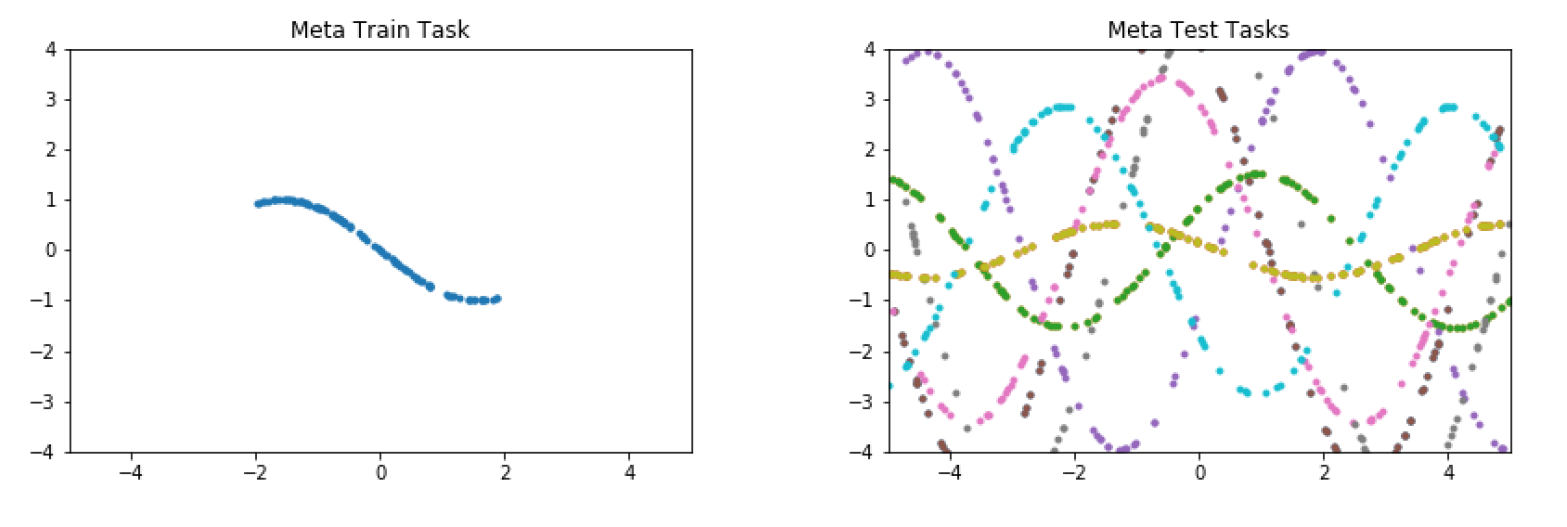
\includegraphics[width=0.65\linewidth]{./Figures/fig2ab.png}
	\caption{Figure 2a-b from \textcite{bechtle2020metalearning}: Meta-train/test tasks.}
	\label{fig:fig2ab}
\end{figure}

For each update at meta-train time the task function is sampled at random locations (although it is not very clear in the paper whether it is indeed SGD or GD), the parameters $\theta$ are updated given the gradients $\nabla_{\theta}\mathbb{E}_{x,y}\pazocal{L}_{\phi}(y, f_{\theta}(x))$ and then the parameters $\phi$ are updated given the gradients $\nabla_{\phi}\mathbb{E}_{x,y}\pazocal{L}_{T}(y, f_{\theta}(x))$.
In this example $\pazocal{L}_{T}(y, f_{\theta}(x)) = (y - f_{\theta}(x))^2$.

Fig.~\ref{fig:fig2c} shows how the final MSE on the training task (after $100$ gradient steps) changes depending on the loss function it is trained with. 
For example, for the blue line, in order to obtain the y-value corresponding to the value of $200$ in the x-axis we have to train $f_{\theta}$ for $100$ gradient steps with the loss function $\pazocal{L}_{\phi}$ corresponding to the meta-train iteration $200$. 
What is not clear from the paper is whether $M=100$ in Algorithm \ref{algo:ML3} and thus, $\phi$ is updated on the whole chain of $100$ updates of $\theta$, or $M=1$ and thus $\phi$ is updated based on a single update of $\theta$, but in order to produce Fig.~\ref{fig:fig2c} $f_{\theta}$ is trained separately for $100$ iterations.
Finally, the orange line corresponds to the final MSE on the training task if the loss function used is $\pazocal{L}_{T}$ directly. 
Obviously, this MSE does not depend on the meta-train iteration and this is why it is constant.

\begin{figure}[H]
	\centering
	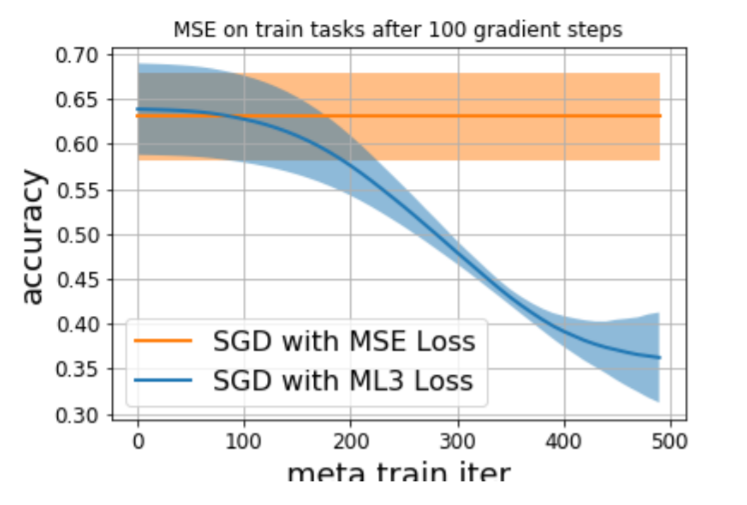
\includegraphics[width=0.65\linewidth]{./Figures/fig2c.png}
	\caption{Figure 2c from \textcite{bechtle2020metalearning}: MSE on train-task for training $f_{\theta}$ with $\pazocal{L}_{T}$ directly (orange) and for training with $\pazocal{L}_{\phi}$ corresponding to the meta-train iteration (blue).
	The uncertainty comes from the initialization of $\phi$ and $\theta$ and the random samples for the train-task. 
	In total $5$ random seeds have been used for obtaining the results.}
	\label{fig:fig2c}
\end{figure}

At meta-test time $10$ test-tasks are drawn and $10$ models are trained independently both with $\pazocal{L}_{T}$ directly and with $\pazocal{L}_{\phi}$ (which has been already trained at meta-train time).
The results are shown in Fig.~\ref{fig:fig2d}. 
\begin{figure}[H]
	\centering
	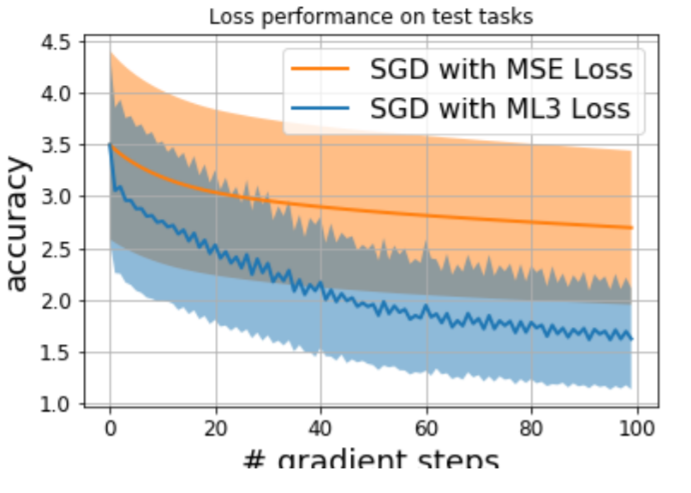
\includegraphics[width=0.65\linewidth]{./Figures/fig2d.png}
	\caption{Figure 2d from \textcite{bechtle2020metalearning}: $\pazocal{L}_{T}$ on $10$ test-tasks for making updates with $\pazocal{L}_{T}$ directly (orange) and for making updates with $\pazocal{L}_{\phi}$ (blue; which has been already trained at meta-train time).
	The uncertainty comes from the initialization of $\theta$, the random test-tasks and the random samples for the test-tasks. 
	In total $5$ random seeds have been used for obtaining the results.}
	\label{fig:fig2d}
\end{figure}	 

\subsection{Toy example: Shaping loss}

Suppose we have $1000$ samples from $y=sin(vx)$ for $x \in [-1,1]$.
We create a model $f_{\omega}(x) = sin(\omega x)$ and we aim to identify the true parameter $v$ with the model parameter $\omega$.
An indicative MSE loss is shown in Fig.~\ref{fig:fig5ab} (note the severe non-convexity).
\begin{figure}[H]
	\centering
	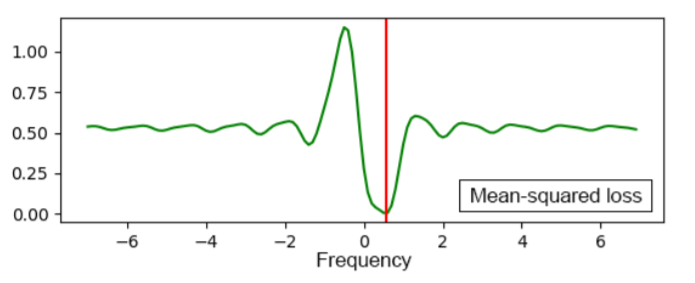
\includegraphics[width=0.7\linewidth]{./Figures/fig5ab.png}
	\caption{Figure 5a bottom from \textcite{bechtle2020metalearning}: Typical MSE loss for learning frequency $v$.}
	\label{fig:fig5ab}
\end{figure}	

Suppose next that we use Algorithm \ref{algo:ML3} for training a meta-loss function $\pazocal{L}_{\phi}$ by using the task-loss $\pazocal{L}_{T} = (\omega - v)^2$, i.e., we assume we know the true $v$. 
Then the obtained loss function $\pazocal{L}_{\phi}$ is convex as shown in Fig.~\ref{fig:fig5at}.
\begin{figure}[H]
	\centering
	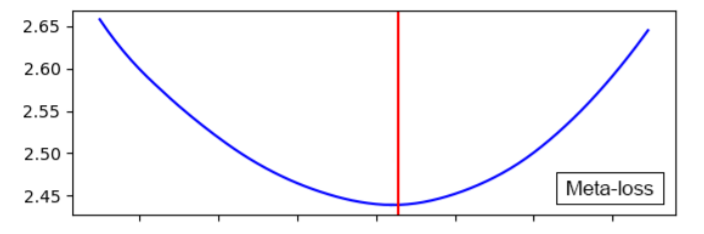
\includegraphics[width=0.7\linewidth]{./Figures/fig5at.png}
	\caption{Figure 5a top from \textcite{bechtle2020metalearning}: Obtained meta-loss function with shaping loss as task-loss.}
	\label{fig:fig5at}
\end{figure}
Further, Fig.~\ref{fig:fig5b} shows the regression loss (most likely they mean the MSE loss $\mathbb{E}_{x}[sin(vx)-sin(\omega x))^2]$) for the case where $\omega$ is updated via the MSE loss (orange), the case where it is updated via the meta-loss obtained with the MSE loss as task-loss (blue) and for the case where it is updated via the meta-loss obtained with the shaping loss as task-loss (green).
The two cases of ML3 are delineated in Algorithm \ref{algo:ML3_shaping_toy}.
It is evident that without shaping the loss landscape, the optimization is prone to getting stuck at a local minimum.

\begin{algorithm}[H]
	\SetAlgoLined
	initialize $\phi$
	
	\While{not converged}{
		initialize $\omega$
		
		sample task samples $x,y$ from T
		
		$\omega \leftarrow \omega - \alpha\nabla_{\omega}\mathbb{E}_{x,y}\pazocal{L}_{\phi}(sin(vx), sin(\omega x))$
		
		\uIf{MSE task-loss (blue)}{
			$\pazocal{L}_{T} = (sin(vx)- sin(\omega x))^2$

		}
		\uElseIf{Shaping loss (green)}{
			$\pazocal{L}_{T} = (v- \omega)^2$
		}
		$\phi \leftarrow \phi - \eta\nabla_{\phi}\mathbb{E}_{x,y}\pazocal{L}_{T}$		

	}
	\textbf{return} meta-loss parameters $\phi$
	\caption{ML3 at meta-train: toy example}
	\label{algo:ML3_shaping_toy}
\end{algorithm}
\begin{figure}[H]
	\centering
	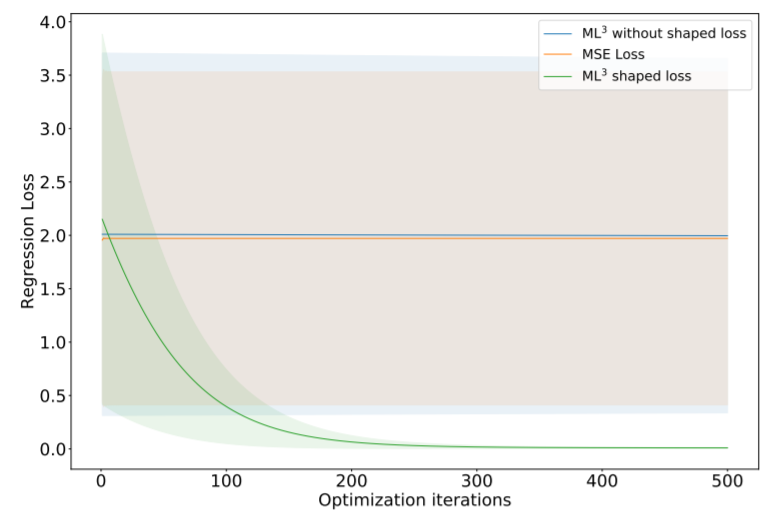
\includegraphics[width=0.7\linewidth]{./Figures/fig5b.png}
	\caption{Figure 5b from \textcite{bechtle2020metalearning}: MSE loss at meta-test time for 3 cases of loss functions (see also Algorithm \ref{algo:ML3_shaping_toy}).}
	\label{fig:fig5b}
\end{figure}

It seems that when the task-loss is so pathological, trying to learn a meta-loss based on it will not help at meta-test time.
As a final note, it does not seem that we can use the learned loss function of this example for test-tasks different than the train-task. 
It was just a toy example.

\subsection{Shaping loss via physics prior for inverse dynamics learning}
Consider the dynamical system
\begin{equation}\label{eq:dyn_system}
	M(q)\ddot{q}+F(q,\dot{q}) = u
\end{equation}
where data for $q,\dot{q},\ddot{q},u$ are provided. 
Indicative ways to learn the map $u \mapsto q,\dot{q},\ddot{q}$ include estimating $M(q)$ from analytical expressions (reference provided in the paper), using a black box map, and using a parametrized inertia matrix $M_{\theta}(q)$ (see \cite{lutter2019deep}).
The latter uses a physics-based MSE loss defined using Eq.~\eqref{eq:dyn_system}.

For improving sample efficiency \textcite{bechtle2020metalearning} proposes to learn a meta-loss $\pazocal{L}_{\phi}$ by using Algorithm \ref{algo:ML3} with task-loss given as $\pazocal{L}_{T} = (M(q)-M_{\theta}(q))^2$, where $M(q)$ (seems to be; it is not very clear) the analytical estimate mentioned above (see Algorithm \ref{algo:ML3_shaping_physics}).
Thus, it acts as a physics-based prior for learning the loss.
What is not very clear in the paper is whether $(M(q)-M_{\theta}(q))^2$ is added to the MSE loss to form the task-loss (like in Eq.~\eqref{eq:total_task}) or the task-loss is equal to just $(M(q)-M_{\theta}(q))^2$.
From the paper the latter seems true, but then how is $M_{\theta}(q)$ faithful to the data as well?

\begin{algorithm}[H]
	\SetAlgoLined
	initialize $\phi$
	
	\While{not converged}{
		initialize $\theta$
		
		sample task samples $q,\dot{q},\ddot{q},u$ from T
		
		$\theta \leftarrow \theta - \alpha\nabla_{\theta}\mathbb{E}_{q,u}\pazocal{L}_{\phi}(u, M_{\theta}(q)\ddot{q}+F(q,\dot{q}))$
		
		\uIf{MSE task-loss (blue)}{
			$\pazocal{L}_{T} = (u - M_{\theta}(q)\ddot{q}-F(q,\dot{q}))^2$
			
		}
		\uElseIf{Shaping task-loss (green)}{
			$\pazocal{L}_{T} = (M(q)-M_{\theta}(q))^2$
		}
		$\phi \leftarrow \phi - \eta\nabla_{\phi}\mathbb{E}_{q,u}\pazocal{L}_{T}$		
		
	}
	\textbf{return} meta-loss parameters $\phi$
	\caption{ML3 at meta-train: shaping loss via physics prior}
	\label{algo:ML3_shaping_physics}
\end{algorithm}

In Fig.~\ref{fig:fig5c} the regression loss is shown for the case where $\theta$ is updated via the MSE loss (orange), via the meta-loss learned with MSE as task-loss (blue) and via the meta-loss learned with the physics prior as task-loss (green).
The two cases of ML3 are delineated in Algorithm \ref{algo:ML3_shaping_physics}.
\begin{figure}[H]
	\centering
	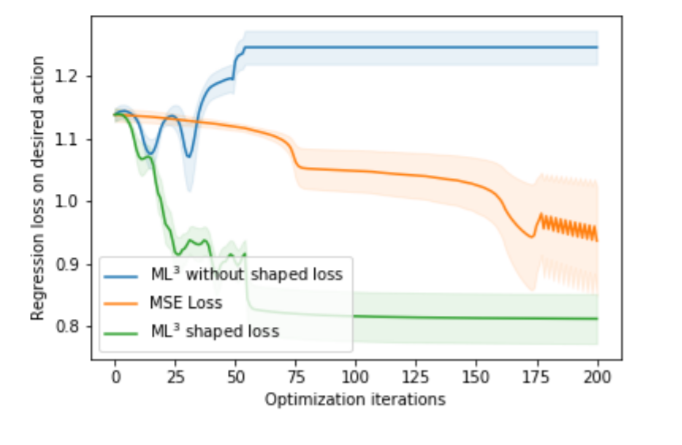
\includegraphics[width=0.7\linewidth]{./Figures/fig5c.png}
	\caption{Figure 5c from \textcite{bechtle2020metalearning}: MSE loss at meta-test time for 3 cases of loss functions.}
	\label{fig:fig5c}
\end{figure}



%%%%%%%%%%%%%%%%%%%%%%%%%%%%%%%%%%%%%%%%%%%%%%%%%%%%%%%%%%%%%%%%%%%%%%%%%%%%%%%%%%%%%%%%%%%%%%%%%%%%%%%%%	

%\section*{Appendix}
\newpage	
\printbibliography[heading=bibintoc,title={References}]
	
\end{document}